%!TEX ROOT = ./main.tex

\section{Experimental Evaluation}\label{sec:experiments}


\begin{table*}
	\large
	\centering
	\caption{List of runtimes for different case-studies
		\textmd{Runtimes (in seconds) for computing open-loop controllers over the corresponding product spaces using ALTRO ($T_{AL}$), number of input-state pairs of finite-state abstraction for local ABCD ($N_l$), abstraction and synthesis times for computing local feedback controllers using SCOTS ($T_{l}^{abs}$ and $T_{l}^{syn}$, respectively), number of input-state pairs of finite-state abstraction for global ABCD ($N_g$), abstraction and synthesis times for computing a global controller for the product system using SCOTS ($T_{g}^{abs}$ and $T_{g}^{syn}$, respectively). For local ABCD, the reported numbers correspond to the maximum value among all of the agents.}
		\label{tab:runtimes}
	}

	\renewcommand{\arraystretch}{1.2}
	\setlength{\tabcolsep}{0.7em} % for the horizontal padding
	%\resizebox{1\columnwidth}{!}{
		\begin{tabular}{l|c|ccc|ccc}
			\toprule
			Case-studie&\multicolumn{1}{c}{Global planning}&
			\multicolumn{3}{|c}{Local ABCD}&\multicolumn{3}{|c}{Global ABCD}\\
			
			&$T_{AL}$&$N_l$&$T_{l}^{abs}$&$T_{l}^{syn}$&$N_g$&$T_g^{abs}$&$T_g^{syn}$\\
			\midrule
			
			\multirow{1}{*}{\rotatebox{0}{Multi-drone path planning}} & $125$ & $1.15\times 10^8$ & $47.66$  & $7.9$& $2.73\times 10^{104}$&OOM&OOM \\
			
			\midrule
			
			\multirow{1}{*}{\rotatebox{0}{Crane and vehicle}} & $0.65$ & $8.56\times 10^{8}$&$511$  & $91$&$2.16\times10^{18}$&OOM&OOM\\
			
			\midrule
			
			\multirow{1}{*}{\rotatebox{0}{Lane merging}} & $100$ & $1.01\times 10^8$&$37.60$  & $ 9.51$&$3.84\times 10^{65}$&OOM&OOM\\
			\midrule
			\multirow{1}{*}{\rotatebox{0}{Multi-drone formation control}} & $163$ & $4.02\times 10^8$&$69.78$  & $13.6$&$3.7\times 10^{59}$&OOM&OOM\\
			\bottomrule
	\end{tabular}%}
\end{table*}


%\MS{List the specifications of the cluster machine/laptop with which we have run our experiments.}
We evaluate a prototype implementation of ALg.~\ref{alg:main}
on two examples. 
The design of nominal controller has been performed on a laptop with core i7-4510u CPU at 3.10GHz, with 8GB of
RAM.
The formal controller synthesis has been performed
on a cluster with 4 Intel Xeon E7-8857 v2 CPUs (48 cores in total) at 3GHz, with 1.5TB of
RAM. %\MS{TODO: adding a table with complete information regarding sizes and times for all of the examples}

We consider two distinct types of problems, and demonstrate how they can be solved using our approach. In all of our examples, robots and obstacles are located over two-dimensional space. Table~\ref{tab:runtimes} demonstrates  runtimes of different stages for each of the experiment. For local ABCD, the reported numbers correspond to the maximum value among all of the agents. This is sensible because feedback controllers for different agents can be computed independently over different machines. Notice that higher number of input-state pairs does not necessarily result in higher runtime for local ABCD as number of transitions and features of the parallel implementation can play a role. Further, Fig.~\ref{fig:box_plot} illustrates variations of runtimes among different agents for every experiment except the crane and vehicle example for which variance is too high because of different dynamics. Note that using global ABCD, memory requirement exceeds our system's limit (1.5TB of RAM) for all of the experiments. %\MS{For reporting number of input-state pairs and runtimes of local ABCD we could report total, average or maximum values; currently, Tab.~\ref{tab:runtimes} contains maximum values (taken over all of the agents, corresponding to multi-machine implementation), while total and average values are reported in the body of the paper. Data will be unified once the decision is made.}
%Note that while reported numbers for local controller synthesis correspond to the total runtimes over all of the robots, significant reduction would be expected if abstraction and synthesis phases were parallelized.
%\begin{huge}



\begin{figure*}[t]
    \large
     \centering
     \begin{subfigure}[b]{0.24\textwidth}
         \centering
         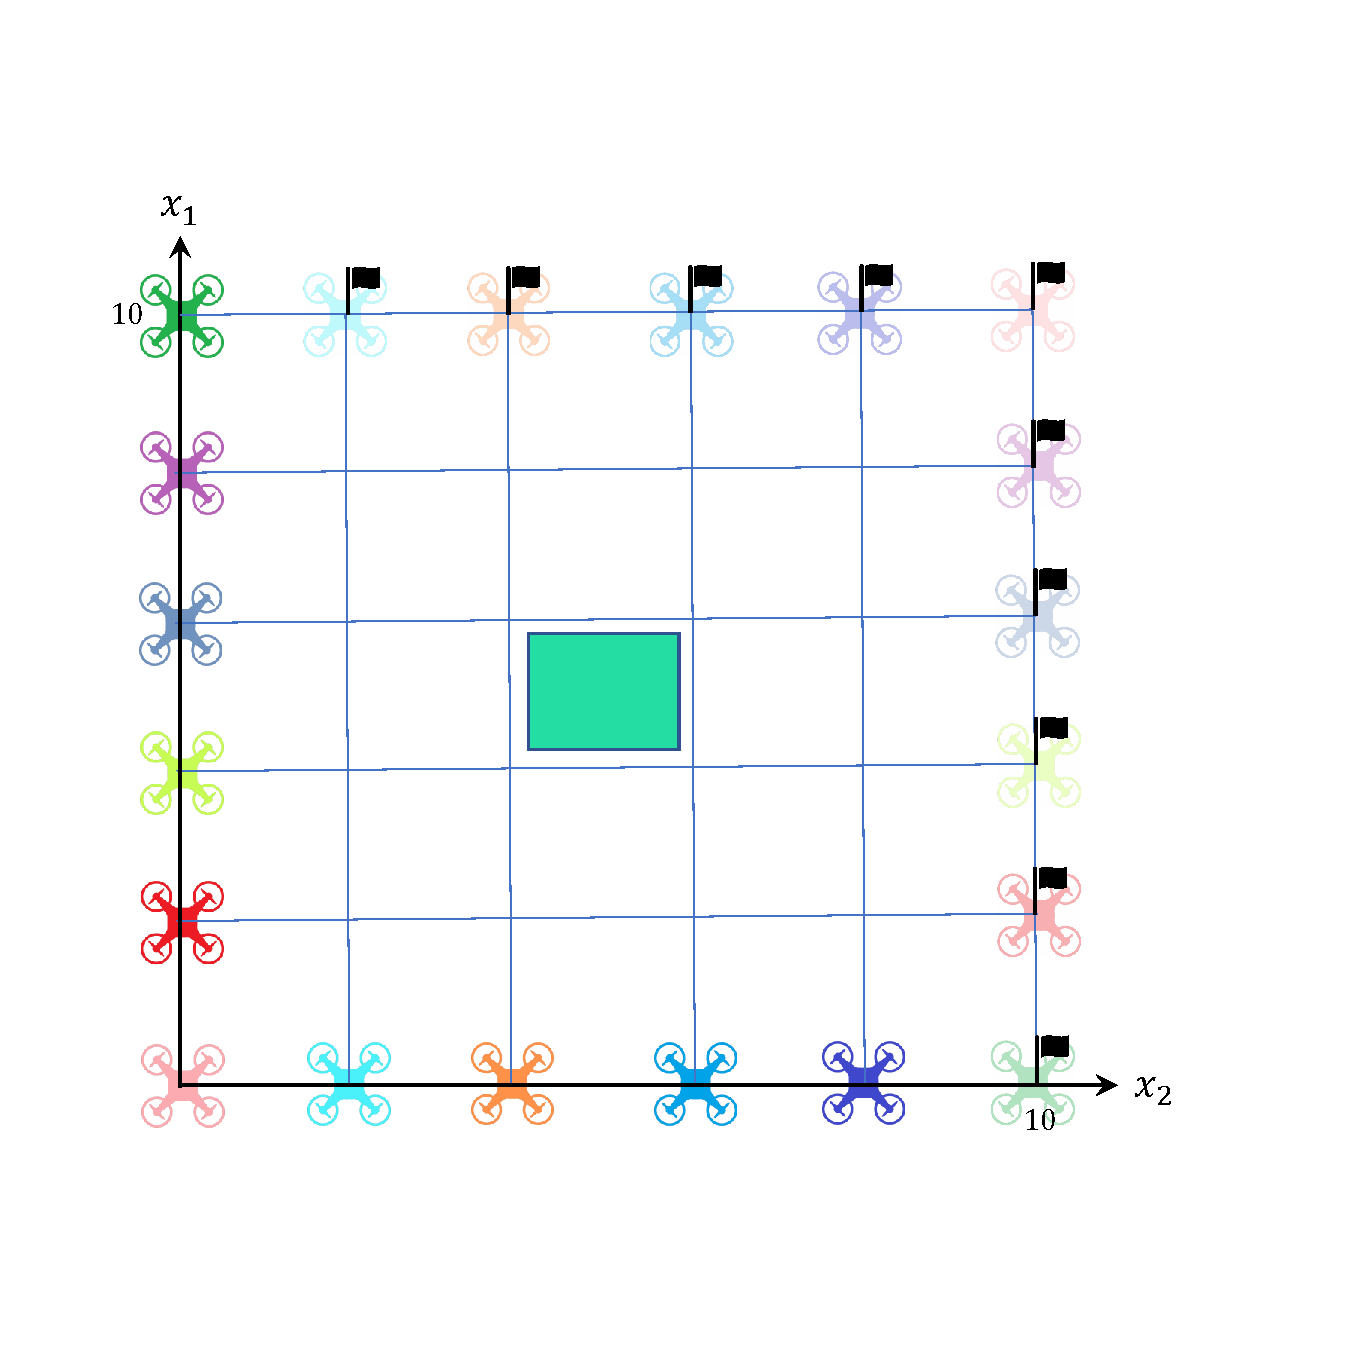
\includegraphics[width=\textwidth]{figures/MA1.pdf}
         \caption{}
         \label{fig:MA}
     \end{subfigure}
     \hfill
     \begin{subfigure}[b]{0.5\textwidth}
         \centering
         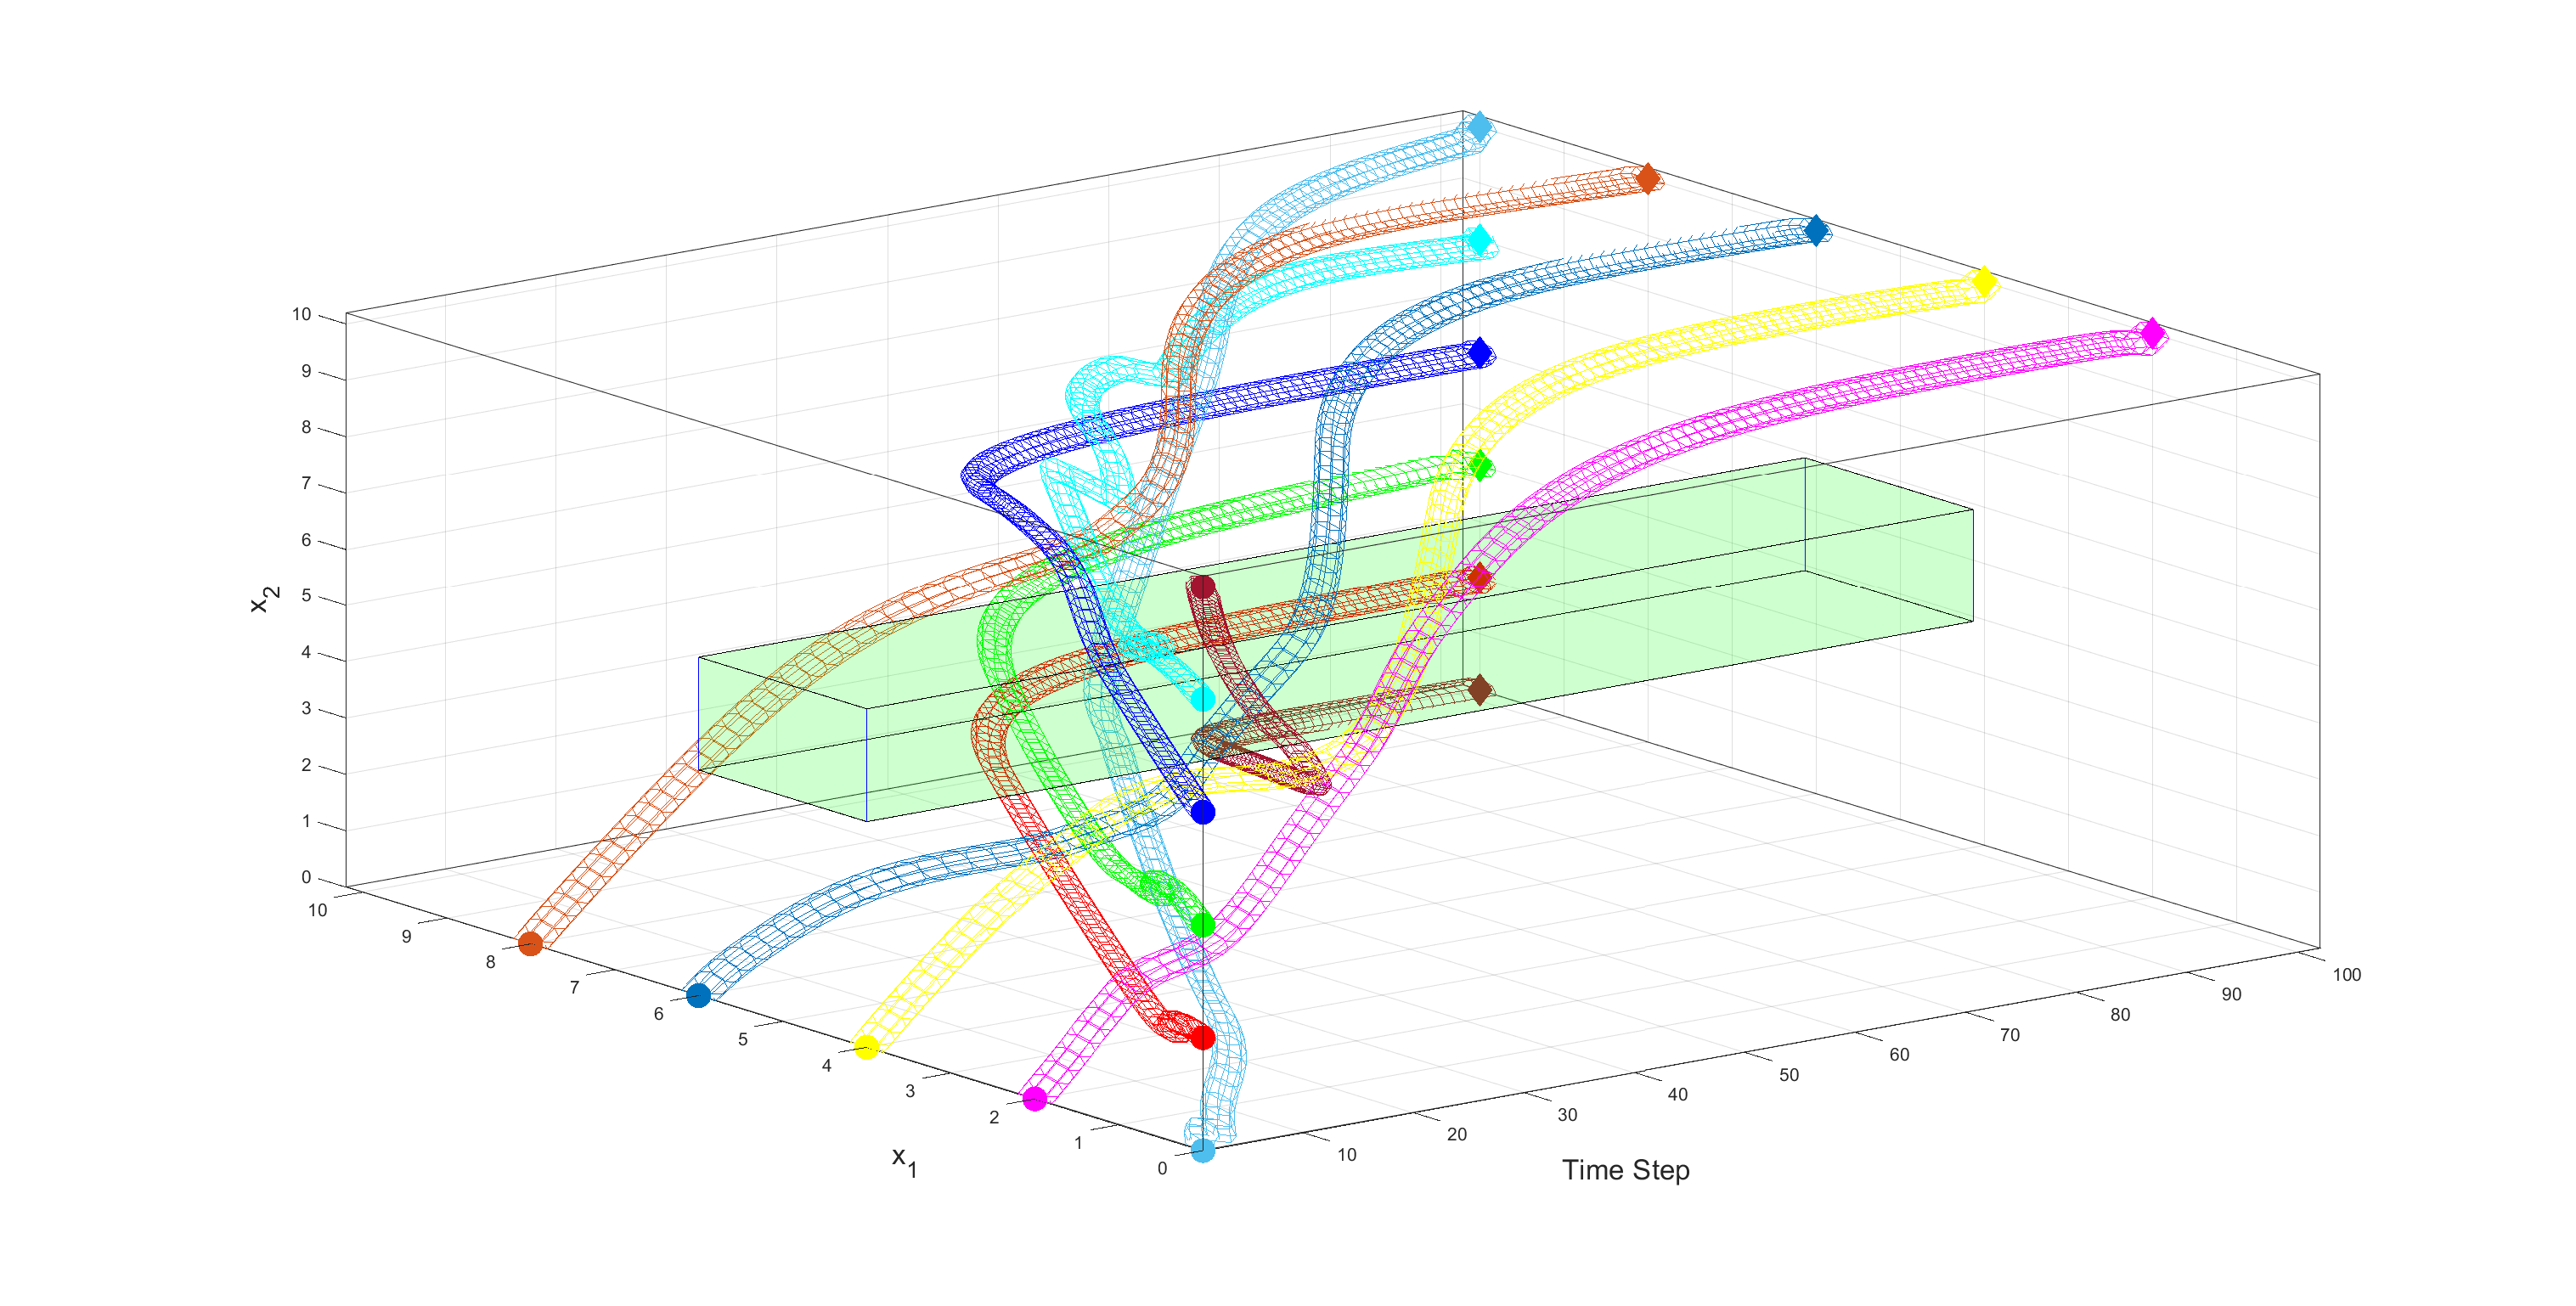
\includegraphics[width=\textwidth]{figures/tubes10.eps}
         \caption{}
         \label{fig:3dtubes}
     \end{subfigure}
     \hfill
     \begin{subfigure}[b]{0.24\textwidth}
         \centering
         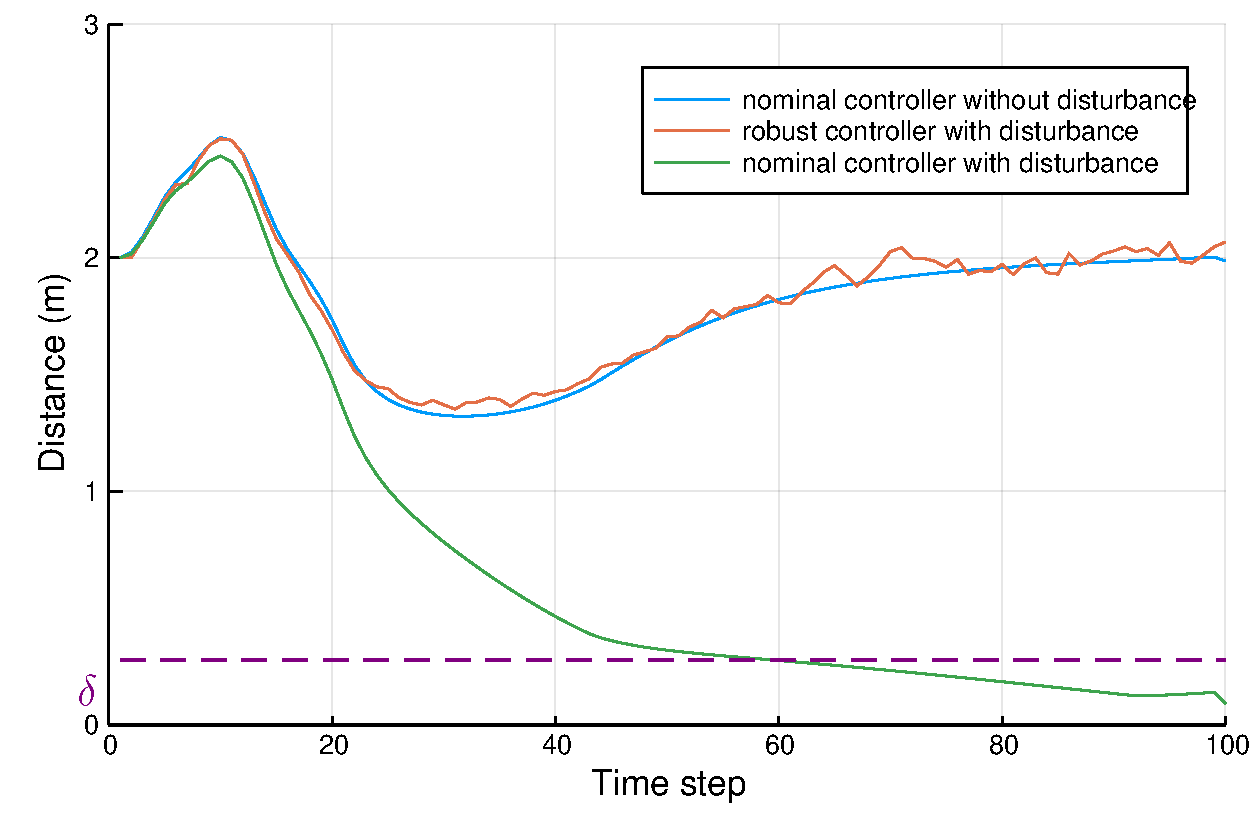
\includegraphics[width=\textwidth]{figures/dist_path_planning.pdf}
         \caption{}
         \label{fig:multi_drone_distance}
     \end{subfigure}
        \caption{(a) The mission map for the multi-drone path planning example (b) Time-state space illustration of tubes enclosing nominal trajectories for the multi-drone path planning (c) Performance of open-loop and feedback controllers in regulating distance between drones for disturbance-free and perturbed situations for the multi-drone path planning example}
        \label{fig:three figures}
\end{figure*}

%\end{huge}
\subsection{Local reach-avoid problems for each robot}
\label{sec:local reach-avoid}

We first consider situations when the robots have got their individual reachability specifications, and they need to ensure a minimum safe distance from each other and the obstacles.
We show how this case can be captured using the problem description outlined in Sec.~\ref{sec:problem}.

Suppose $\set{\Sigma^i=(X^i,x_\init^i,U^i,W^i,f^i)}$ is a set of control systems, $\goal^i\subseteq X^i$ is the individual goal states and $\delta \in \mathbb{R}_{>0}$ is a safety margin.
%(We could also consider obstacles in the agent' own state spaces, in which case we had to additionally introduce safety margins in the state spaces.)
%Without loss of generality, we assume that every robot is moving in the two-dimensional space.
Suppose the specification requires that each robot $\Sigma^i$ eventually reaches $\goal^i$ while avoiding obstacle $\obs\subseteq \reals^2$ and collision with robots by the margin $\delta$.
This specification can be expressed as a reach-avoid specification of the product system $\Sigma^\times$, as per the required form given in Sec.~\ref{sec:problem}, as follows:
\begin{itemize}
	\item The goal set $\goal\subseteq X^\times$ is defined as $\goal \coloneqq \goal^1\times \ldots \times \goal^N \subseteq X^\times$, and
	\item The static obstacle $\avoid\subseteq X^\times$ is defined as 
		\begin{align}
			&\avoid \coloneqq\nonumber\\ 
				&\Set{ x^\times\in X^\times | 
					\begin{array}{c}
						\exists i\in [1;N]\;.\; D(x^i,\obs) \leq \delta\\
						\vee\\
						 \exists (i,j)\in [1;N]\times [1;N]\;.\;\\ d\left(x^i,x^j\right)\leq\delta
					\end{array}},
		\end{align}
	where $x^i$ denotes the component of $x^\times$ corresponding to the $i^{th}$ subsystem, $d(\cdot,\cdot)$ denotes a predicate for measuring the geometric distance between positions of two systems located in two-dimensional space, $D(\cdot,\cdot)$ denotes a predicate for measuring the geometric distance between position of one system and an obstacle located in two-dimensional space.
\end{itemize}

Once the sets $\goal$ and $\avoid$ are obtained as above, we can use Alg.~\ref{alg:main} to find the set of feedback controllers $\set{C^i}$.

In this category of problems, we consider the following three examples.

%\textcolor{red}{
\subsubsection{Multi-drone path planning}\label{sec:Multirobot}
In this example, we consider a planning scenario for ten identical drones ($N=10$). A set of initial and target states for each drone are specified and depicted in Fig.~\ref{fig:MA}. The drones must avoid hitting a physical obstacle that is depicted with green square in Fig.~\ref{fig:MA}. %A physical obstacle is added to the problem over the $2D$ plane, depicted in Figure~\ref{fig:MA} with a yellow circle. 
The threshold for minimum distance from the obstacle and other drones is chosen to be $\delta=\begin{bmatrix}0.28&0.28\end{bmatrix}^T$. %and $\delta_{obs}=\begin{bmatrix}2&2\end{bmatrix}^T$.
The control objective is to synthesize a feedback controller for each drone so that in the presence of (bounded) disturbance, beginning from the specified initial state, the corresponding target state is reached within a finite horizon, while avoiding collision with other drones and the physical obstacle at every time point. 

Every drone is modeled as tuple $\Sigma^i=(X,x_\init^i,U,W,f^d_\tau)$. %The set of state variables $X$ consists of $x_1$, $x_2$ and $x_3$ which denote position in $2D$ plane and movement angle, respectively. The set of input variables includes $u_1$ and $u_2$ which represent linear and angular speeds of each robot. 
Continuous time dynamics for each drone takes the form
\begin{equation*}\label{eq:unicycle_ss}
	f^{d}(x(t),u(t))=
	\begin{bmatrix}
		\dot{x_1}\\
		\dot{x_2}\\
		\dot{x_3}
	\end{bmatrix}=
	\begin{bmatrix}
		u_1cos(x_3)\\
		u_1sin(x_3)\\
		u_2
	\end{bmatrix}.
\end{equation*}
where $x_1$ and $x_2$ denote the drone's position in two-dimensional space, $x_3$ denotes the rotational angle, and $u_1$ and $u_2$ represent control inputs for each drone. Choosing a sampling time $\tau=0.1$, nominal dynamics $f^d_\tau$ can be characterized uniquely. %Further, the output mapping is defined as
%\[
%h^d(x(t))=\begin{bmatrix}
%	x_1\\x_2
%\end{bmatrix}.
%\]
%In the above equation, $u_1(t)$ and $u_2(t)$ denote linear and angular speeds at time $t$, respectively. Further, $x_1(t)$, $x_2(t)$ specify position in $x-y$ plane and $x_3$ denotes the angle at time $t$. 


%According to our proposed scheme, we first use ALTRO to design a centralized nominal controller for the product state and input space that satisfies the specification in Equation~\eqref{eq:spec} in the absence of disturbance ($W=\{0\}$). 
\begin{figure}[h]
	\centering
	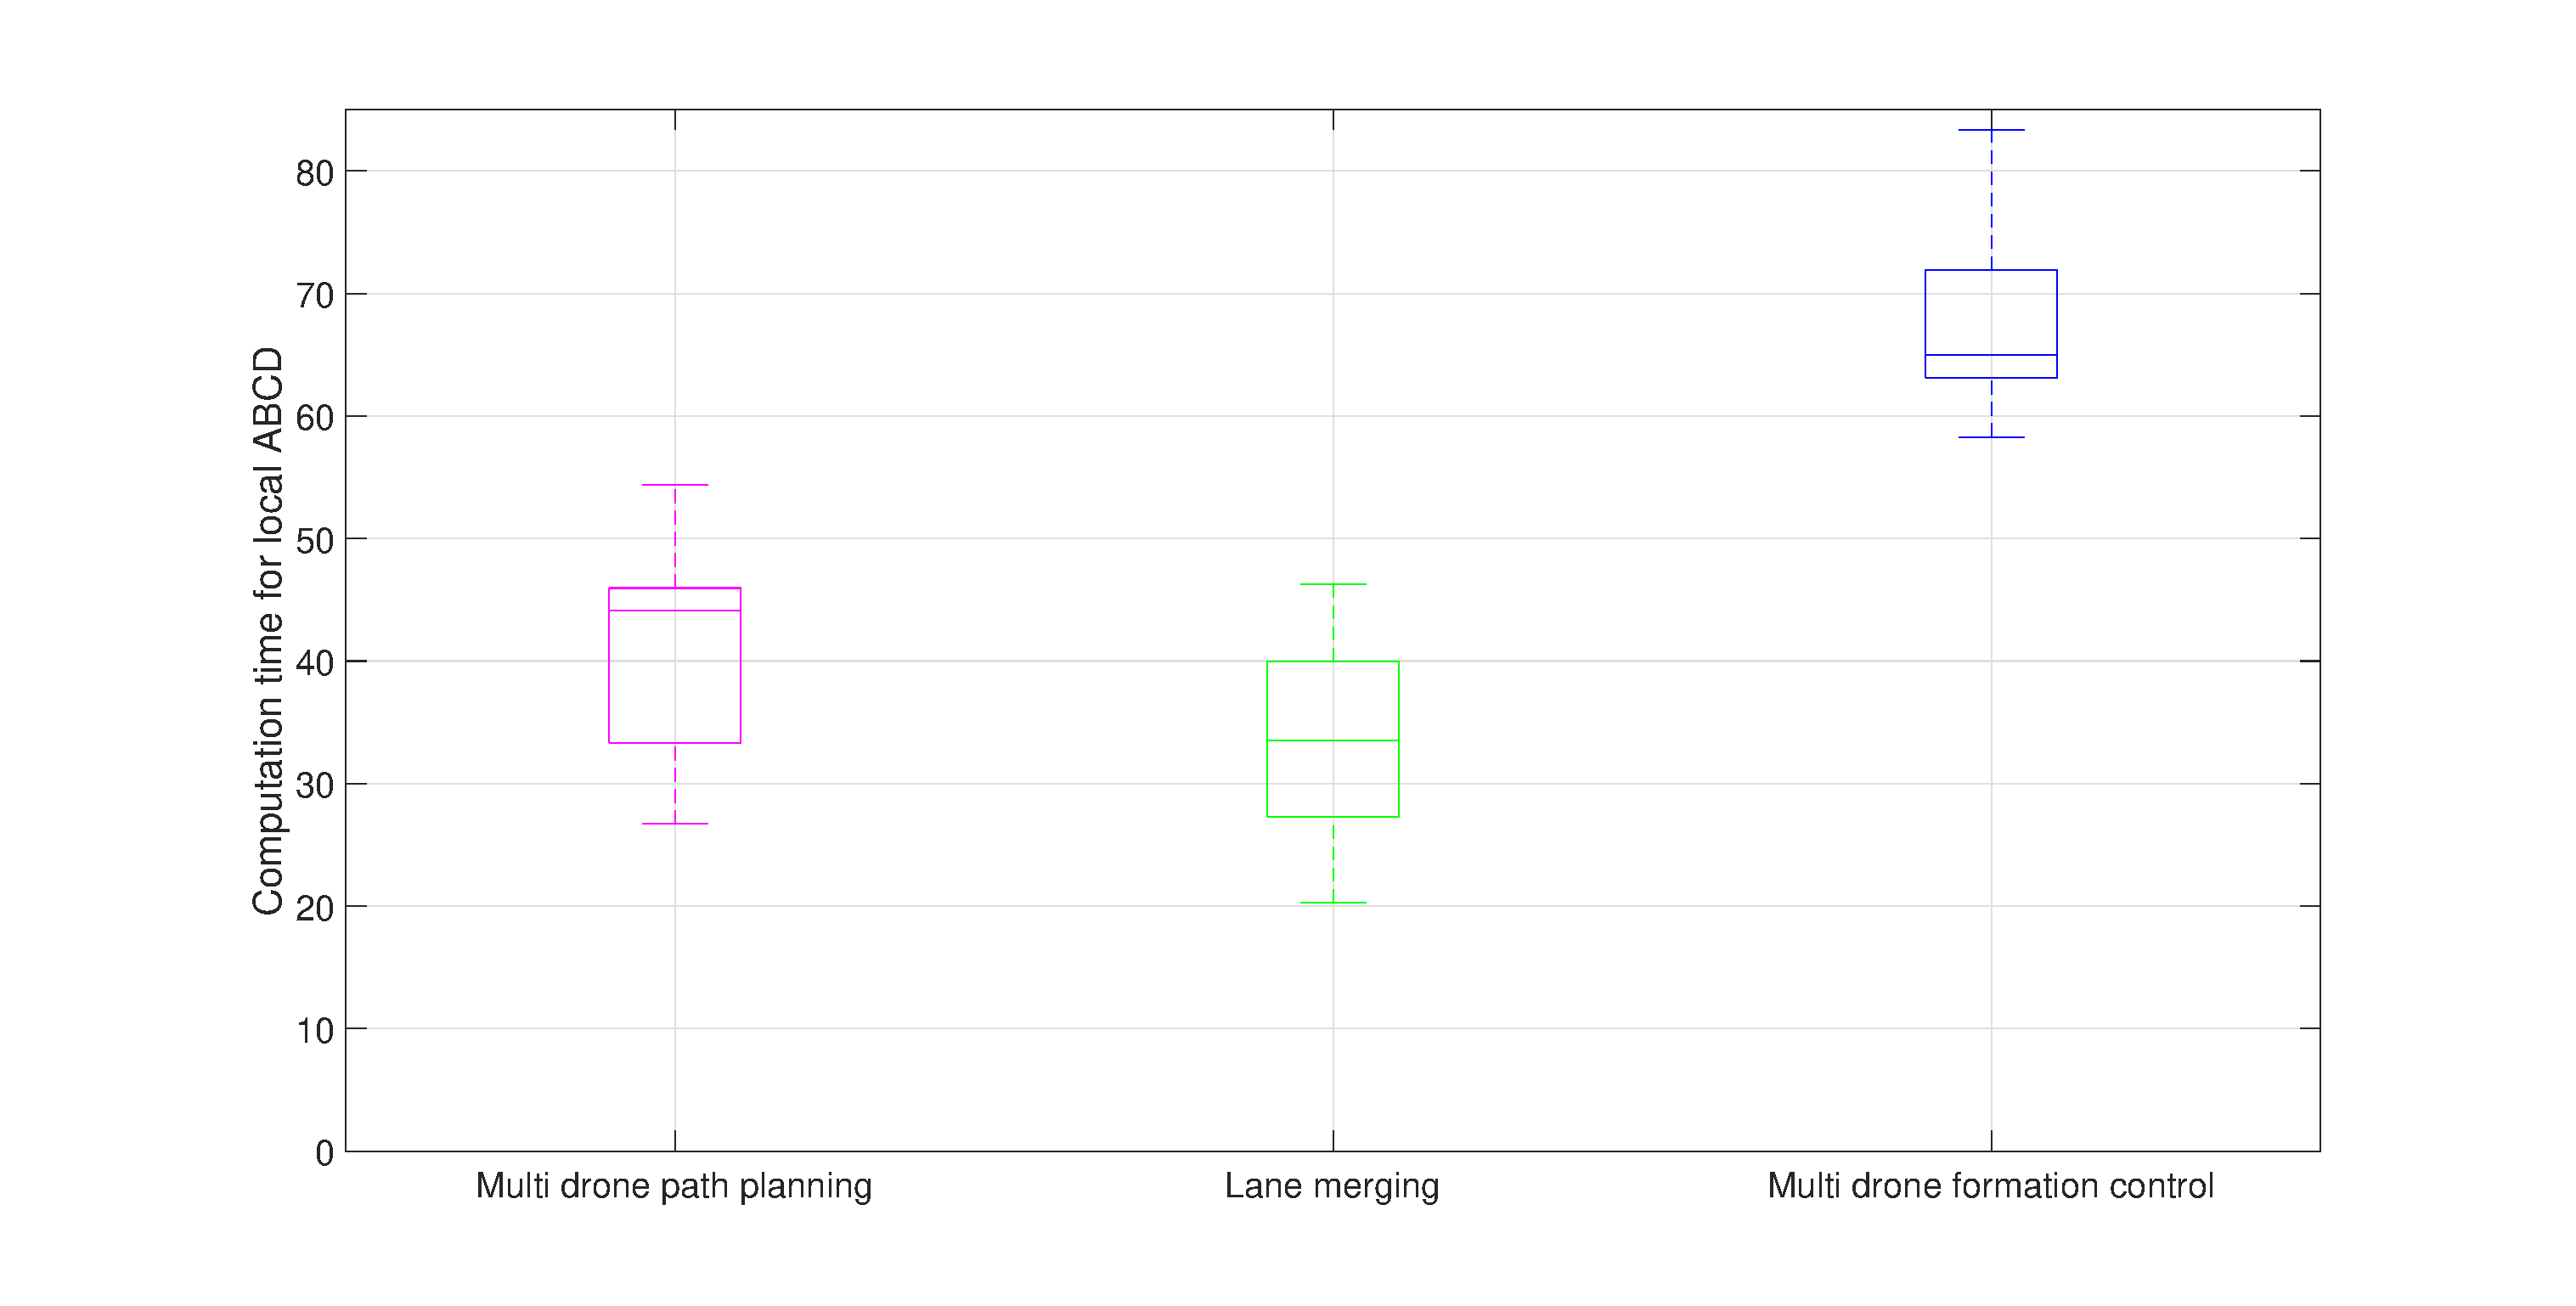
\includegraphics[width=0.45\textwidth]{figures/Box_plot.eps}
	\caption{Variations of runtimes among different agents for different experiments using local ABCD}
	\label{fig:box_plot}
\end{figure}
Selecting the horizon length as $T=102$, %and sampling time $\tau=0.1$. 
ALTRO computes a valid open-loop trajectory %$x_{nom}$
in $125$ seconds for the product system with $30$ state and $20$ input variables.  %Next, we show how to synthesize local feedback controllers that guarantee satisfaction of specifications in the presence of disturbance. %hereeeThe open-loop trajectories generated by ALTRO ($\set{(x_{0_\nom}^i,\ldots,x_{K_\nom}^i)}_{i\in [1;N]}$) are depicted in solid in Figure~\ref{fig:MA}. Note that the guarantee that open-loop controller gives is only valid in the absence of disturbance. In Figure~\ref{fig:MA}, dotted trajectories correspond to the first and the second robot's paths in $2D$ plane when constant additive disturbance $w=\{\begin{bmatrix}0.03,0.03,0.03\end{bmatrix}\}$ is being applied throughout the whole horizon. It can be noticed that they collide with each other before reaching their corresponding target sets. Next, we show how to synthesize local controllers that guarantee satisfaction of specifications in the presence of disturbance. \MS{1) Use dashed/dotted for trajectories with added disturbance. 2) use $x_1$ and $x_2$ instead of $x$ and $y$ for different axes 3) don't draw the outer circle.}

%We augment each open-loop trajectory with time 
%We construct a tube around the (nominal) trajectory produced by ALTRO with the width vector
%The tube with the width $\varepsilon=\begin{bmatrix}0.16&0.16&0.32\end{bmatrix}^T$ is constructed around the nominal trajectory has.
%Note that $\delta_{col} > \varepsilon$.
 %We use SCOTS in order to synthesize (local) feedback controllers that guarantee reachability and obstacle/collision avoidance in the presence of bounded disturbance such that 
 
 %To implement step~\ref{step:tracking} of Alg.~\ref{alg:main}, we need to design local feedback controllers that can keep the agent's trajectories inside $\varepsilon$-balls defined around the nominal trajectories computed by ALTRO. 
 Fig.~\ref{fig:3dtubes} gives time-space illustration for the safe tubes around the nominal trajectories. We want to robustify the nominal controller against disturbances with $|W|\leq \begin{bmatrix}0&0.025&0.025\end{bmatrix}^T$. We consider state and input spaces to be $X=[-1,11]^2\times[-2,3.3]$ and
$U=[-2.4,2.4]^2$, respectively. Choosing  $\eta_{X}=\begin{bmatrix}0.02&0.02&0.02\end{bmatrix}^T$, $\eta_{U}=\begin{bmatrix}0.3&0.3\end{bmatrix}^T$ and $\varepsilon=\begin{bmatrix}0.16&0.16&0.18\end{bmatrix}^T$, Tab.~\ref{tab:runtimes} illustrates list of runtimes and number of input-state pairs corresponding to local and global ABCD. Noticeably, for number of agents $N>1$, memory requirement for global ABCD exceeds our limits (1.5TB of RAM). 
%results in $\hat X$ and $\hat U$ with $9.61\times 10^7$ and $289$ points. We compute the transition system over the inter-tube space characterized by $\varepsilon=\begin{bmatrix}0.16&0.16&0.18\end{bmatrix}^T$, which results in finite-state transition system with $4.0\times 10^5$ points. Given the above settings, SCOTS computes abstraction in $340$ seconds ($34.0$ seconds in average) and synthesis in $73$ seconds ($7.3$ seconds in average). %(the ones with red dashed circles around them in Fig~\ref{fig:MA}). 
%It can be noticed that success in restricting the trajectories generated under the worst-case disturbance within the tubes guarantees a collision-free mission.
%Fig~\ref{fig:blowup} illustrates the fact that increasing number of agents ($N$) causes an exponential blow-up in the number of transitions if we wanted to solve the given reach-avoid problem over the product state and input spaces. However, since we compute tracking controllers locally, our method experiences linear blow-up as $N$ increases.


On the other hand, using ALTRO alone would not provide guarantee against bounded disturbance.  %By allowing disturbance to take non-zero values, there is no guarantee that the open-loop trajectories are followed.
Fig.~\ref{fig:multi_drone_distance} illustrates performance of open-loop and feedback controllers on regulating distance between the two of drones with and without disturbance. As expected, in the absence of disturbance open-loop controller suffices and distance between the two drones (shown in solid blue) does not go below the defined threshold. Next, we consider the case when constant additive disturbance vectors $\begin{bmatrix}0 &0.025&0.025\end{bmatrix}^T$ and $\begin{bmatrix}0 &-0.025&-0.025\end{bmatrix}^T$ are being applied to the two drones throughout the whole horizon. It can be noticed that applying the open-loop controller causes that distance between the two drones (shown in solid green) to go blow the predefined threshold. However, the feedback controller is capable of maintaining distance (shown in solid red) within the safe region when the same disturbance is being applied.


%In this example, we are focusing on number of robots. This example consist of 10 identical unicycle model. Each unicycle should start from its own initial point and reach target set which is shown in Fig. \ref{fig:MA} with green points and red points. while it avoids obstacles and collision with other agents. Unicycle model is described in below.
%\begin{equation}\label{eq:unicycle_ss}
%	f^{u}(x(t),u(t))=
%	\begin{bmatrix}
%	\dot{x_1}\\
%	\dot{x_2}\\
%	\dot{x_3}
%	\end{bmatrix}=
%	\begin{bmatrix}
%	u_1cos(x_3)\\
%	u_1sin(x_3)\\
%	u_2
%	\end{bmatrix}.
%\end{equation}
%In Eq. \ref{eq:unicycle_ss} $u_1$ is linear speed and $u_2$ is  angular speed and $x_1$ and $x_2$ represents positions and $x_3$ is the angle. Here goal of the problem is designing a controller which satisfy the specifications which mentioned in sec. \ref{sec:Problem_statement}. For this purpose, According to sec.\ref{sec:nominal trajectory} at first we combine all of unicycle dynamics to create a centralized model of the centralized system. The centralized system has $10\times3$ dimension for state space and $10\times2$ dimension for input space. For collision avoidance and obstacle avoidance we use $\delta_{col}=1.5$ and $\delta_{obs}=2$ and we use euclidean distance as a metric for distance in 2D space. In this step, we solved mentioned problem with ALTRO with sample time 0.05 and 200 points for trajectory. Computation takes 138 seconds. Result of ALTRO is illustrated in fig \ref{fig:MA}. 
%In next step we synthesize close loop controller using ABCD with $\varepsilon=[0.16,0.16,0.16]$.  As we mentioned in Prob. \ref{alg:abcd-with-time-for-tracking} we are going to to design a controller that is able to track the trajectory with $\varepsilon$ distance in every time step which is also robust to the disturbance .\MZ{Here we can split the centralized system to 10 separate system and design a close loop controller for each one of them separately.} In order to do this step, we select $\varepsilon$ in a way that it satisfies $\delta_{col} > 2\sqrt{\varepsilon_x^2+\varepsilon_y^2}$ (since tubes should not intersect with each other). Then we are able to design a controller guaranteeing the specifications for each agent independently using Alg. \ref{alg:abcd-with-time-for-tracking} and SCOTS. We select parameters in this way:\\
%$\widetilde{X}=[-1:11]*[-1:11]*[-\pi,\pi]*[0,1]$\\
%$U=[-3,3]*[-3,3]$\\
%$\eta_{\widetilde{X}}=[0.04,0.04,0.04,0.05]$\\
%$\eta_{U}=[0.6,0.6]$\\
%number of states = about $7*10^7$\\
%reduced number of states = about $7*10^7$\\
%number of inputs =121\\
%
%Abstraction in total for 10 systems takes about 12 minutes(average 100 seconds for each system) and synthesizing controller takes about 2 minutes(near 15 seconds for each system). Controller designed in this way is able to overcome bounded additive disturbance $|w|\leq[0.03,0.03,0.03]$ (for all of unicycles). Nominal controller which is produced by ALTRO with presence of this disturbance will be pushed outside of $\epsilon$ tube and also as it shown in the Fig.\ref{fig:MA}, trajectory 1 and 2 will have collision with this value of disturbance. 




 %Figure~\ref{fig:inv_pend} demonstrates variations of disturbance limit under which SCOTS is able to find a controller for different tube width. %It can be observed that by increasing the tube width, SCOTS is able to synthesize a controller for larger disturbance levels. Figure~\ref{fig:invpend_traj} demonstartes trajectories of the system  \eqref{eq:inv_pend_ssq} governed by controllers synthesized by ALTRO and SCOTS under appliance of constant disturbance vector \MS{$[??,??]$}. As expected, the controller designed by ALTRO is not able to tackle disturbance, while using the controller generated by SCOTS, the trajectory remains within the desired bound.

%\begin{figure}\label{fig:inv_pend}
%	\includegraphics[]{}
%	\caption{Variations of disturbance limit for which SCOTS is able to find a controller with tube size}
%\end{figure}
%\begin{figure}\label{fig:invpend_traj}
%	\includegraphics[]{}
%	\caption{}
%\end{figure}
%\textcolor{red}{
\subsubsection{Crane and Vehicle}
\label{subsec}
The goal of this example is to study performance of our method for controlling a number of robots with different dynamics. %Consider a production line wherein a crane (modeled as a cart-pole system) puts some items at certain points and a forklift is in charge of picking these items up. It is assumed that at its lowest height the crane's hook is positioned such that the forklift cannot pass. In particular, Fig.~\ref{fig:cr_and_lft_2} shows a scenario wherein the crane (initially positioned toward left of the boom) needs to unload at the other end of the boom. At the same time, the forklift (initially positioned near the right end of the boom) needs to pick some item locating near the left end of the boom. The goal is to control both the crane and the forklift so that the forklift reaches the object without colliding with the crane. 
We model the crane and vehicle by tuples $\Sigma^1=(X^1,x_\init^1,U^1,W^1,f_\tau^c)$ and $\Sigma^2=(X^2,x_\init^2,U^2,W^2,f_\tau^l)$, respectively. The crane is modeled as cart-pole system taking the form \cite{Barto1983}:
\begin{align*}
	\ddot{\theta} &= \frac{M_tg\sin(\theta) - \cos(\theta)(F + M_pl \dot{\theta}^2 \sin(\theta))}{l(4/3 M_t- M_p \cos^2(\theta))}=f^c_1(\theta,\dot{\theta},F)\\
	\ddot{z}&= \frac{F + M_pl \dot{\theta}^2 \sin(\theta)-M_pl \ddot{\theta} \cos(\theta)}{M_t}=f^c_2(\theta,\dot{\theta},F),
\end{align*}
where
\begin{itemize}
	\item[] $g=-9.8$ $m/s^2$ is the acceleration of gravity,
	\item[] $M_c=1$ kg is the cart mass,
	\item[] $M_p=0.1$ kg is the pole mass,
	\item[] $M_t=M_c+M_p$ denotes the total mass,
	\item[] $l=0.5$ m is the half-pole length.
\end{itemize}
Further, cart's position, pole's angle and input force to the cart are denoted by $x_1^{(1)}=z$, $x_3^{(1)}=\theta$ and $u^{(1)}=F$, respectively. Continuous-time dynamics of the crane is of the following form:
 %for which the set of state variables $X^1$ consists of $x_1^{(1)}$, $x_2^{(1)}$, $x_3^{(1)}$ and $x_4^{(1)}$ denoting (linear) position and speed of the cart and (angular) position and speed of the pole, respectively. The set of input variables includes $u_1^{(1)}$ which represents linear acceleration of the cart. Finally, crane's dynamics takes the form for an inverted pendulum (see, e.g., \cite{barto1983neuronlike}) and can be written as
\[f^{c}(x^{(1)}(t),u^{(1)}(t))=\begin{bmatrix}
	\dot{x}_1^{(1)}\\
	\dot{x}_2^{(1)}\\
	\dot{x}_3^{(1)}\\
	\dot{x}_4^{(1)}
\end{bmatrix}=\begin{bmatrix}
\dot{z}\\
\ddot{z}\\
\dot{\theta}\\
\ddot{\theta}
\end{bmatrix}=
\begin{bmatrix}
	x_2^{(1)}\\
	f^c_1(x_3^{(1)},x_4^{(1)},u^{(1)})\\
	x_4^{(1)}\\
	f^c_2(x_3^{(1)},x_4^{(1)},u^{(1)})\\
\end{bmatrix}.\]
%with
%\begin{align}
%	f^c_2(x{(1)},u^{(1)})=\frac{g\;\sin(x_3^{(1)})}{}
%\end{align}
%\MS{what are $f^c_1$ and $f^c_2$?}
%The output mapping for the crane is defined as
%\[
%h^c(x^{(1)}(t))=\begin{bmatrix}
%	x_1^{(1)}+l \sin(x_3^{(1)})\\
%	y_1+l \cos(x_3^{(1)})
%\end{bmatrix},
%\]
%where, $y_1>0$ is a constant that denotes the cart's height from the ground.
The vehicle's continuous-time dynamics takes the form of
\[f^{l}_{con}(x^{(2)}(t),u^{(2)}(t))=\begin{bmatrix}
\dot{x}_1^{(2)}\\ \dot{x}^{(2)}_2 \end{bmatrix}=\begin{bmatrix} x^{(2)}_2\\ u^{(2)} \end{bmatrix},
\]
where $x_1^{(2)}$ and $x_2^{(2)}$ denote the vehicle's position and speed and $u^{(2)}$ represents the vehicle's control input (acceleration). Fixing the sampling time $\tau=0.1$, one can derive $f^c_\tau$ and $f^l_\tau$. %The output mapping for the crane is defined as
%\[
%h^l=\begin{bmatrix}
%	x_1^{(2)}\\
%	y_2
%\end{bmatrix},
%\]
%where, $y_2>0$ is a constant that denotes the height of the forklift's head with respect to the ground.

%As promised, we use ALTRO in the first step to generate a valid trajectory for the case that $W=\{0\}$. 
There is no obstacle for this example and for minimum distance between the crane and the vehicle we choose $\delta=\begin{bmatrix}0.035&0.2\end{bmatrix}^T$. Fixing the horizon length to $T=70$, ALTRO was capable of generating a valid nominal trajectory in $0.65$ seconds. Fig.~\ref{fig:cr_and_lft} (\textbf{left}) demonstrates snapshots of the produced trajectory. Surprisingly enough, applying (constant) additive disturbance $W=\begin{bmatrix}0&0.05&0&0\end{bmatrix}^T$ (to the cart-pole system) causes collision between the crane and vehicle before the end of the mission (Fig.~\ref{fig:cr_and_lft} (\textbf{right})).

In the next step, we use SCOTS in order to compute a feedback controller tolerating additive disturbance $|W^1|\leq\begin{bmatrix}0&0.05&0&0\end{bmatrix}^T$ for the crane and $|W^2|\leq\begin{bmatrix}0&0.1\end{bmatrix}^T$ for the vehicle. %We note that the selection of tube sizes need to satisfy the following inequality:
%\[ \delta_{col}> \varepsilon_{1}^{(1)} + l\times\varepsilon_{3}^{(1)} + \varepsilon_{1}^{(2)},\]
%where $\varepsilon_{1}^{(1)}$, $\varepsilon_{3}^{(1)}$ denote tube sizes over $x_1^{(1)}$ and $x_3^{(1)}$, $l$ denotes the length of the rope between the cart and the hook and $\varepsilon_{1}^{(2)}$ denotes the tube size over $x_1^{(2)}$. 
We choose state and input spaces for the crane to be $X^{1}=[-0.195,5.49]\times[-1.99,4.37]\times[1.20,4.68]\times[-5.44,5.28]$ and $U^{1}=[-7,7]$, respectively. For the vehicle, we set $X^{2}=[3,9]\times[-3,1.995]$ and $U^{2}=[-3,3]$. %Next, we augment both dynamics with time and 
We choose state and input partition sizes $\eta_{{X}}^{1}=\begin{bmatrix}0.015&0.035&0.016&0.064\end{bmatrix}^T$, $\eta_{U}^1=0.2$,  $\eta_{{X}}^2=\begin{bmatrix}0.01&0.015\end{bmatrix}^T$ and $\eta_{U}^2=0.1$. %These selections yield discretized models with state and input spaces having $2.5\times 10^9$ and $71$ points for the crane, and $2\times 10^5$ and $61$ points for the vehicle. 
Next, we limit both of the state spaces into tubes constructed around the open-loop trajectories with sizes specified as $\varepsilon^{1}=\begin{bmatrix}0.135&0.385&0.176 &0.768\end{bmatrix}^T$ and $\varepsilon^{2}=\begin{bmatrix}0.08&0.12\end{bmatrix}$. %This reduces size of state spaces into $1.2\times 10^7$ and $1.5\times 10^4$ for the crane and vehicle, respectively. 
%Given the above settings, SCOTS was able to compute abstraction in $511$ and $0.22$ seconds for the crane and the vehicle, respectively. Scots performs synthesis in $91$ and $0.037$ seconds for the crane and the vehicle, respectively.
Tab.~\ref{tab:runtimes} illustrates list of runtimes and number of input-state pairs corresponding to local and global ABCD. Noticeably, for the cart-pole model, memory requirement for global ABCD exceeds our limits (1.5TB of RAM). On the other hand, using ALTRO alone would not provide guarantee against bounded disturbance (Fig~\ref{fig:cr_and_lft}, \textbf{right}). 

			
%\begin{figure}[t]
%	\centering
%	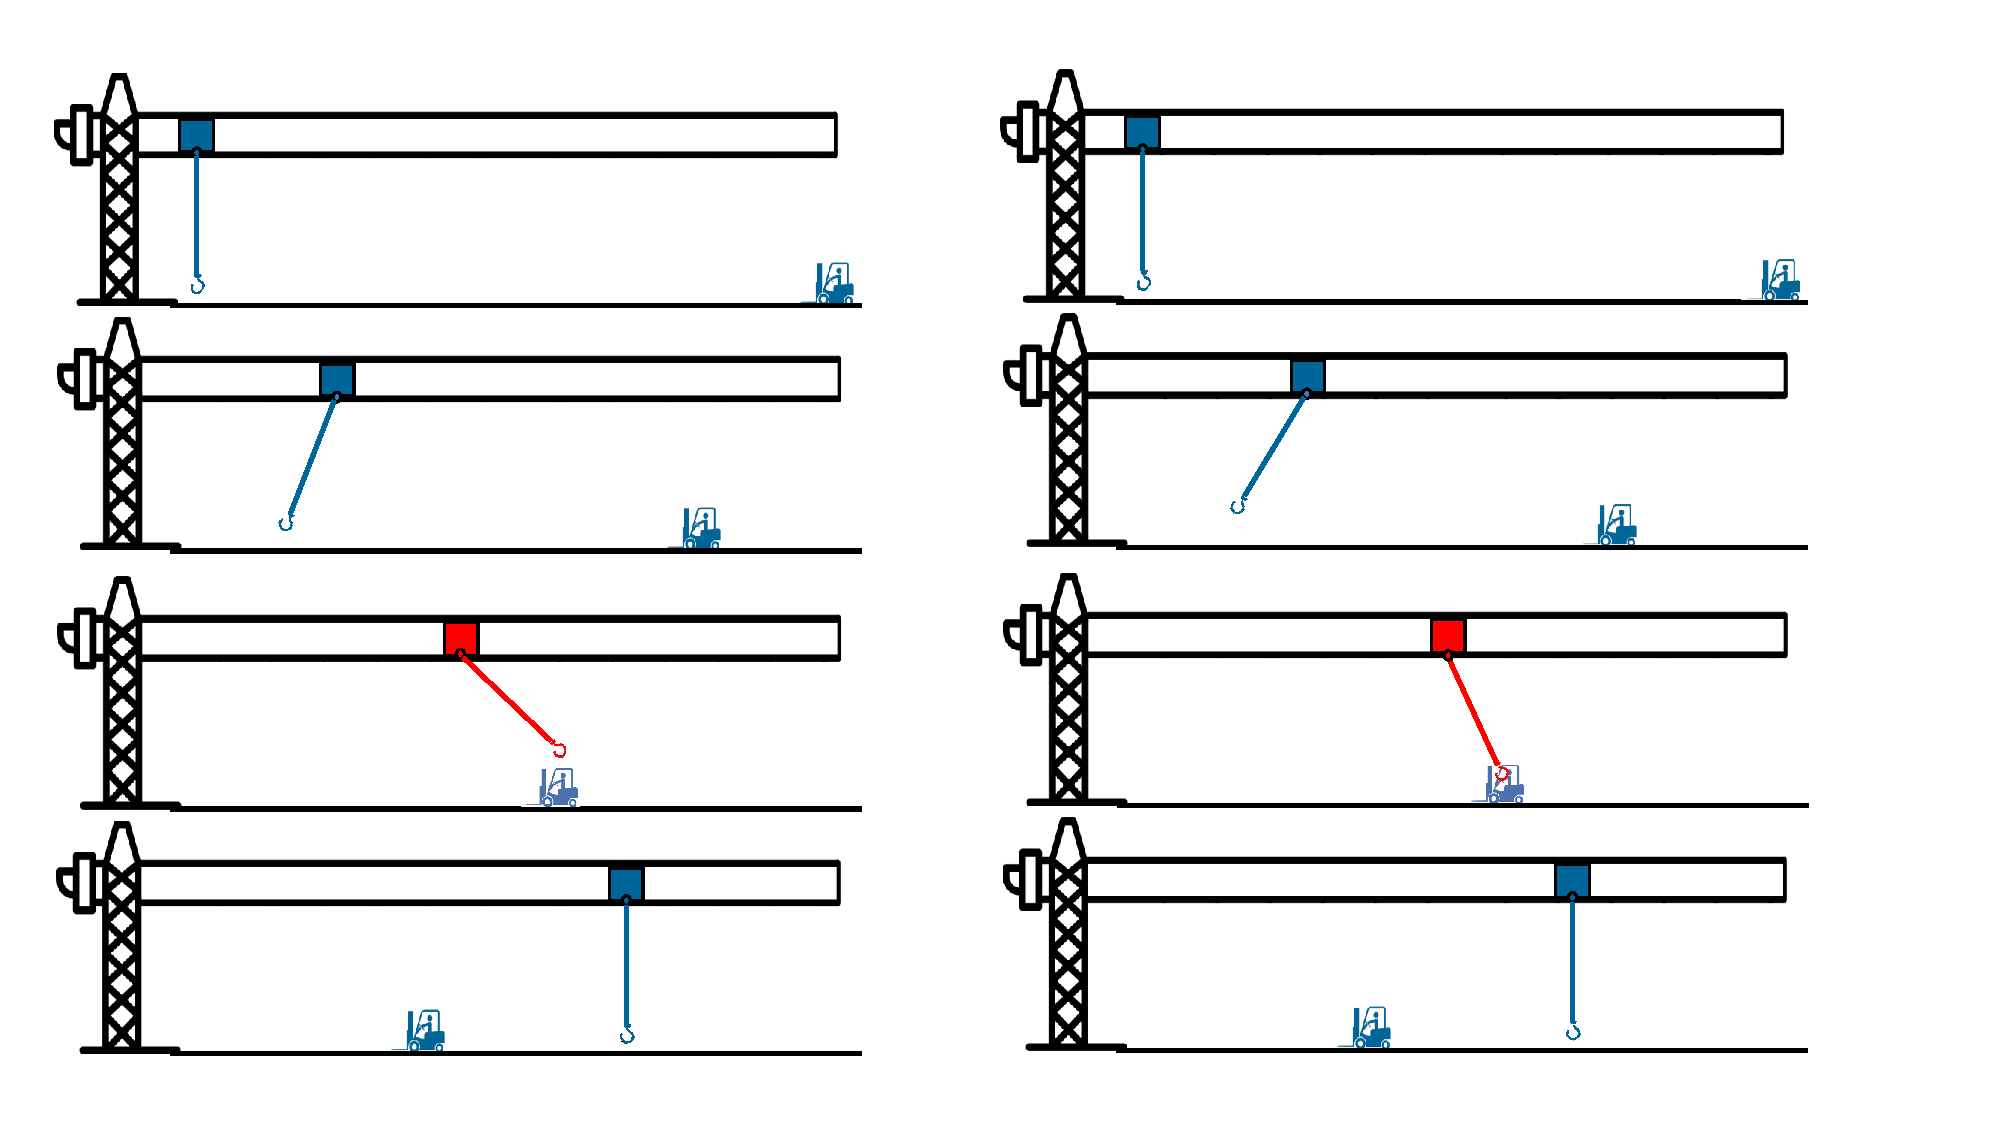
\includegraphics[width=0.45\textwidth]{figures/crane_and_forklifter.pdf}
%	\caption{Illustration of the trajectories generated by the open-loop controller for the crane and vehicle example under disturbance-free (\textbf{left}) and perturbed (\textbf{right}) situations} 
%	\label{fig:cr_and_lft_2}
%\end{figure}


%In this example, we show the method can handle multiple heterogeneous dynamical systems. This example is Modelling a special situation in a factory(shown in fig \ref{fig:cr_and_lft}) . Assume there is a crane and and a forklift. Each one of them should reach their destination without having any accident(satisfying specs). The Crane position will change from 0 to 5 and the forklift from 9 to 4.  Here we model the forklift using $\begin{bmatrix} \dot{x_1}\\ \dot{x_2} \end{bmatrix}=\begin{bmatrix} x_2\\ u \end{bmatrix}$ ($x_1$ and $x_2$ are representing position and velocity) and for the crane we use inverted pendulum model with exactly same configuration in \cite{barto1983neuronlike}: \\ 
%\[\begin{bmatrix}
%\dot{x}\\
%\Ddot{x}\\
%\dot{\theta}\\
%\Ddot{\theta}
%\end{bmatrix}=\begin{bmatrix}
%\dot{x_1}\\
%\dot{x_2}\\
%\dot{x_3}\\
%\dot{x_4}
%\end{bmatrix}=\begin{bmatrix}
%x_2\\
%g(x_3,x_4,u)\\
%x_4\\
%f(x_3,x_4,u)\\
%\end{bmatrix}\]
%
%where $x$ represent position of the cart  and $\theta$ is angle of the pole, f and g are non-linear functions. The process of controller design is similar to Sec. \ref{sec:MultiAgent}; At first we find a nominal trajectory with ALTRO with required specifications then we robustifing it using our method with modified ABCD.\\
%In this example we do not have any static obstacle, but for collision avoidance we use euclidean distance as the metric with $\delta=0.4$ for measuring distance between crane and forklift. We consider hook of crane as a point mass with a radius and forklift as several point mass on circumference of it, So we consider minimum distance between the hook and points of the forklift as the distance. ALTRO solve this trajectory generation problem using sampling time =0.1 and number of points=40 in 10.7 seconds.\\
%to guarantee collision avoidance specification we should select tube sizes to satisfy:
%\[ \delta_{col}> \varepsilon_x + l*\varepsilon_\theta + \varepsilon^\prime_x\]
%where $\varepsilon_x$ and $\varepsilon_\theta$ are tube sizes for position and angle in crane model (cart pole) and l is the length of the joint and $\varepsilon^\prime_x$ is tube size for position of the forklift.
%In next phase we use finite abstraction with $\varepsilon_x=9*0.015$ and $\varepsilon_\theta=11*0.015$ and $\varepsilon^\prime_x=9*0.015$. It takes about 1000 seconds for crane (cart-pole system) with (1.15)*($10^{11}$) number of input-states pairs and ($7*10^6$)*(71) reduced number of states and synthesis takes 35 seconds. For forklift abstractions abstraction and synthesis will finish in less than a second.\\
%The nominal controller with disturbances $w_1=[0,0.02,0,0]$ for crane and $w_2=[0,0.1]$ for forklift will fail collision specification.
%
%


%} 


\subsubsection{Lane Merging}
Finally, we study a lane merging problem wherein multiple controlled vehicles are driving over two merging lanes (Fig.~\ref{fig:merge}, \textbf{top} frame). A dangerous situation may occur at the merging point of the two lanes if vehicles are not controlled properly. Different variants of this problem has been studied in the literature (see, e.g., \cite{xiao2019merging,xiao2020merging}). Without seeking to optimize fuel consumption or travel time, we set the goal to control the vehicles to pass the merging zone safely. In particular, consider a situation where initially three cars are driving on each of the two lanes (Fig.~\ref{fig:merge}, (\textbf{top})). The control objective for each vehicle is to pass the red dashed line within a finite horizon without hitting the road's sides or colliding with other vehicles. 

%Every vehicle is modeled as tuple $\Sigma=(X,U,W,f^v,Y,h^v)$. 
%Dynamics for each vehicle takes the form
%\begin{equation*}\label{eq:vehicle_ss}
%	f^{v}(x(t),u(t))=
%	\begin{bmatrix}
%		\dot{x_1}\\
%		\dot{x_2}
%	\end{bmatrix}=
%	\begin{bmatrix}
%		u_1\\
%		u_2
%	\end{bmatrix},
%\end{equation*}
%where $x_1$, $x_2$ denote the vehicle's position in $2D$ plane, $u_1$ and $u_2$ represent the vehicle's speed coordinates, respectively. The output mapping is defined as
%\[
%h^v(x(t))=x(t).
%\]
The model for each of the vehicles is the same as the drone model given in Sec.~\ref{sec:Multirobot} ($\Sigma^i=(X,x_\init^i,U,W,f^d_\tau)$). For collision and obstacle avoidance, we choose $\delta=\begin{bmatrix}0.37&0.37\end{bmatrix}^T$. The horizon length is fixed to $T=110$. Given these settings, ALTRO generates a valid nominal trajectory in $100$ seconds. Next, we use SCOTS in order to compute feedback controllers tolerating additive disturbance $|W|\leq\begin{bmatrix}0.03&0.03&0.03\end{bmatrix}^T$. We choose state and input spaces for each vehicle's model to be $X=[-0.5,15]\times[0.1,7.4]\times[-1,0.4]$ and $U=[-0.9,3]\times[-2.1,2.1]$, respectively. State and input partition sizes are chosen as $\eta_{X}=\begin{bmatrix}0.02&0.02&0.02\end{bmatrix}^T$ and $\eta_{U}=\begin{bmatrix}0.3&0.15\end{bmatrix}^T$. %These selections yield discretized models with abstract state and input spaces having $2.1\times 10^7$ and $406$ points. 
Next, we limit the state spaces into tubes constructed around the open-loop trajectories with sizes specified as $\varepsilon=\begin{bmatrix}0.16&0.16&0.16\end{bmatrix}^T$. %This reduces size of state space into $1.9\times 10^5$ (in average). Given the above settings, SCOTS was able to compute abstraction in $159.6$ seconds ($26.6$ seconds in average) and synthesize controllers in $40.8$ seconds ($6.8$ seconds in average).
Tab.~\ref{tab:runtimes} illustrates list of runtimes and number of input-state pairs corresponding to local and global ABCD. Noticeably, for number of agents $N>1$, memory requirement for global ABCD exceeds our limits (1.5TB of RAM). Fig.~\ref{fig:merge} demonstrates snapshots of one sample trajectory when feedback controllers are employed under the presence of disturbance. It should be noticed that using ALTRO alone would not provide guarantee against bounded disturbance.
Fig.~\ref{fig:multi_drone_distance} illustrates the fact that open-loop controller fails in keeping one of the vehicles away from the road's sides under perturbed situation when constant additive disturbance vector $\begin{bmatrix}-0.03 &0.03&-0.03\end{bmatrix}^T$ is being applied throughout the whole horizon. In contrast, emplying feedback controller results in successful lane merging. %Fig.~\ref{fig:multi_drone_distance} illustrates performance of open-loop and feedback controllers on regulating distance between of the vehicles from the road's sides with and without disturbance. In the absence of disturbance open-loop controller is capable of maintaing a minimum distance from the road's sides. Next, we consider the case when constant additive disturbance vector $\begin{bmatrix}-0.03 &0.03&-0.03\end{bmatrix}^T$ is being applied to the vehicle throughout the whole horizon. It can be noticed that applying the open-loop controller causes that distance from the road's side (shown in solid red) becomes smaller than $\delta$. However, the feedback controller is still capable of maintaining distance above the given threshold (shown in solid green).





%
%consider the situation which is found in ref[??]. In this situation we consider 6 numbers of car in two different lanes(merging lane and main lane) . Here the goal is reaching the red line ( x position should get bigger than 15) which is shown in fig ?? while they satisfying specifications ( avoid collision with other cars and border of lanes) .
%Number of cars is fixed it means number of cars not changing during simulation time. but it also doesn't mean all of the cars reach the target at same time.\\
%The problem that we are solving has several differences with the example on the paper. they optimize time and fuel for each car and tehy consider several constraints for speed and positions. they also consider 2d linear model for each car. Here we only try to solve the reachability problem. we consider reach top speed limitation and angle acceleration and lanesborders As constraints. For each car we consider the model represented in eq[6] (same model as multi-car example) which has more dimension and is nonlinear.



\begin{figure}[t]
	\centering
	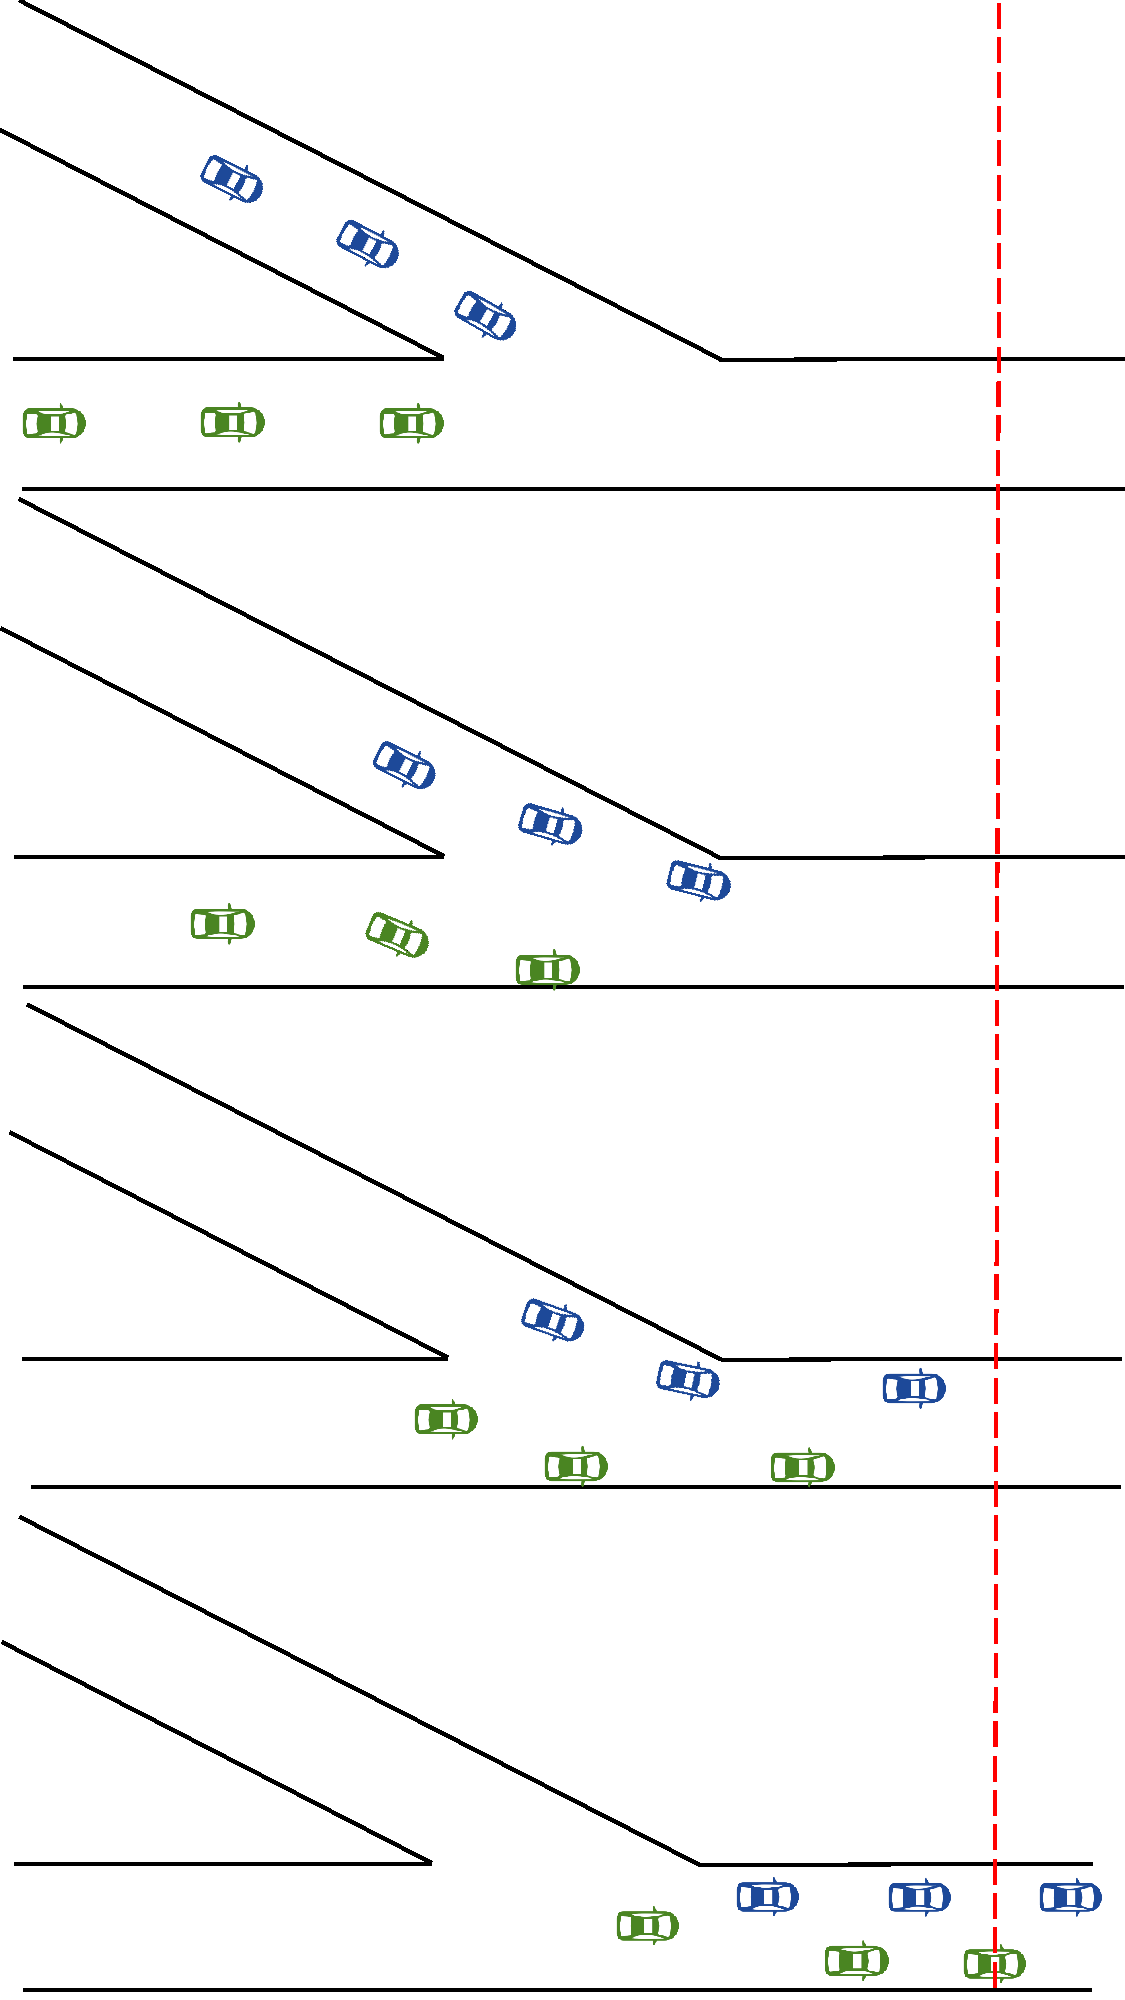
\includegraphics[scale=.2]{figures/merge.pdf}
	\caption{Illustration of a (sample) trajectory generated by formally guaranteed feedback controllers for the lane merging example}
	\label{fig:merge}
\end{figure}

\begin{figure}[t]
	\centering
	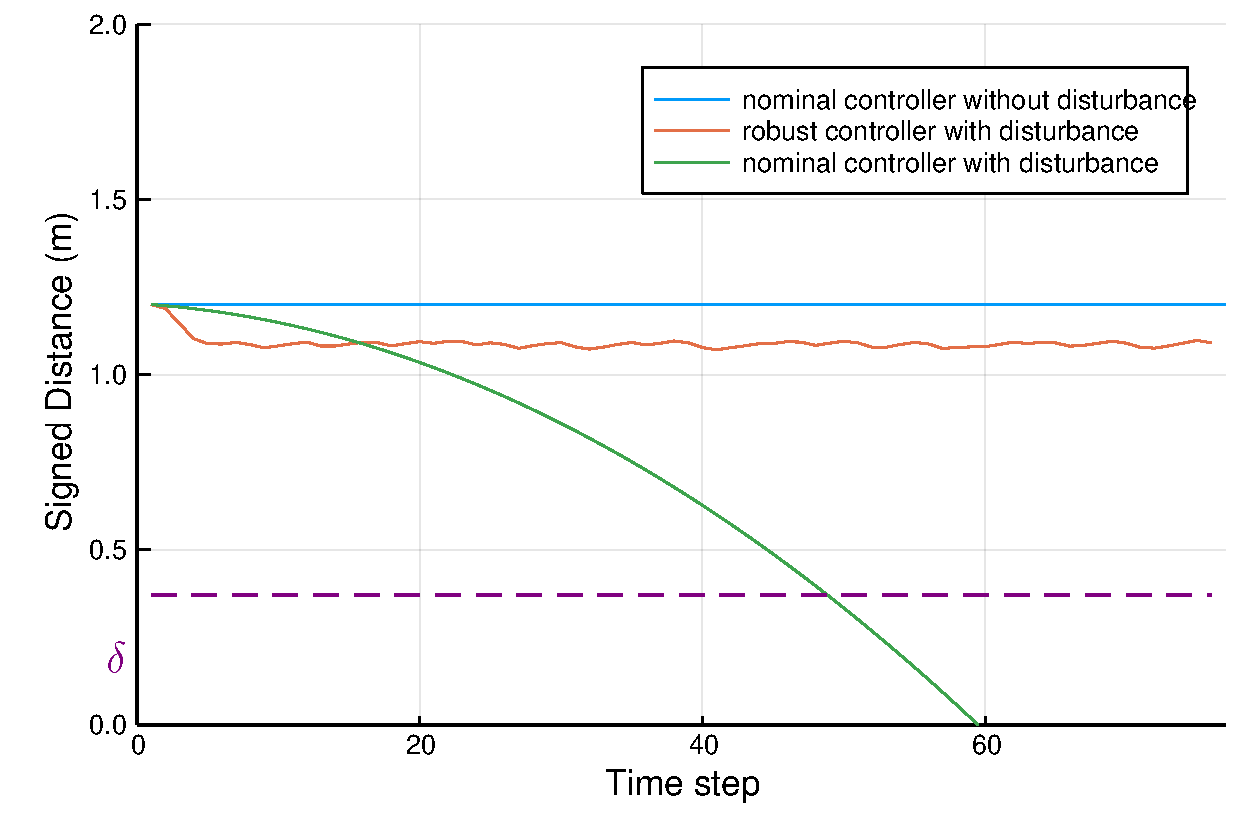
\includegraphics[width=0.45\textwidth]{figures/dist_merging.pdf}
	\caption{Performance of open-loop and feedback controllers in regulating distance between one vehicle and the road side for disturbance-free and perturbed situations for the lane merging example}
	\label{fig:merging_distance}
\end{figure}


\subsection{Global formation control problem}\label{sec:global formation control}

The second category of example, that we are about to present, is about maintaining a global formation while satisfying a set of reach-avoid specifications.
We show how the formation control problem can be expressed using a static obstacle $\avoid$ on the product state space $X^\times$, as required by the problem setup in Sec.~\ref{sec:problem}.

Let us first formalize the notion of formation.
Let $\Set{\Sigma^i=(X^i,x_\init^i,U^i,W^i,f^i)}$ be a set of robots.
A \emph{formation constraint} is a set $\Set{\lambda^{i,j}\in \mathbb{R}}_{i,j\in [1;N]}$ where every $\lambda^{i,j}$ specifies the relative \emph{euclidean} distance between the projections of state of robot $\Sigma^i$ and robot $\Sigma^j$ over the shared output space $Y$.
%(We use euclidean distance to define formation, as opposed to the distance $D$ used in the rest of the paper, to allow rotation of the formation while moving.)

Now suppose $\goal^i\subseteq X^i$ is the individual goal states, $\obs\subset \reals^2$ is a common obstacle in the output space, $\delta \in \mathbb{R}^2_{>0}$ is a safety margin, and $\mu\in \mathbb{R}_{>0}$ is a tolerance margin for the formation constraint.
The formation control problem then asks to generate controllers $\set{C_i}$ such that every robot $\Sigma^i$ eventually reaches $\goal^i$ while avoiding $\obs$ by the margin $\delta$, as well as while making sure that the \emph{euclidean} distance between robot $\Sigma^i$ and $\Sigma^j$ is in the range $\lambda^{i,j} \pm \mu$.
Essentially the tolerance margin $\mu$ is to account for the possible slight deviations due to disturbances experienced by the robots. Notice that since the robots have their own goals, and at the same time they need to ``stay close'' to their neighboring robots in the formation for the entire period, hence they might first need to accompany the other robots to their goals, before being accompanied by them to reach its own goal.

%Let $D_e\colon \mathbb{R}^n\times \mathbb{R}^n\to \mathbb{R}^p_{\geq0}$ denote the euclidean distance.

We can express the formation control problem in the product state space as follows:
\begin{itemize}
	\item The goal set $\goal\subseteq X^\times$ is defined as $\goal \coloneqq \goal^1\times \ldots \times \goal^N \subseteq X^\times$, and
	\item The static obstacle $\avoid\subseteq X^\times$ is defined as 
		\begin{align}
			&\avoid \coloneqq\nonumber\\ 
			&\Set{ x^\times\in X^\times | 
				\begin{array}{c}
					\exists i\in [1;N]\;.\; D(x^i,\obs) \leq \delta\\
					\vee\\
					\exists (i,j)\in [1;N]\times [1;N]\;.\;\\ d\left(x^i,x^j\right)\notin\lambda^{i,j}\pm \mu
			\end{array}},					
		\end{align}
\end{itemize}
where the last disjunction in the definition of $\avoid$ is the restriction required for maintaining the formation, and the rest are same as in Sec.~\ref{sec:local reach-avoid}.
Once the sets $\goal$ and $\avoid$ are obtained as above, we can use Alg.~\ref{alg:main} to find the set of feedback controllers $\set{C^i}$.

%\todo{The example goes here...}
\subsubsection{Multi-drone formation control}
\label{subsec:formation_control}
Consider a formation control scenario where a set of five drones (identically modelled) need to go from a specified start point to a certain destination (both defined over the corresponding state spaces) within a finite horizon, while four of them forming a diamond around a fifth drone (positioned at the diamond's center) at every time point. There are two square-shaped obstacles (defined over the output space) from which the group needs to keep a certain minimum distance at all of the time points. %As mentioned before, to check the formation the relative positions between the $i^{th}$ and $j^{th}$ drones is measured by euclidean norm ($d_e^p(.,.)$) whereas collision/obstacle avoidance is checked by the infinity norm$d^p(.,.)$.

The model for each of the drones is the same as the drone model given in Sec.~\ref{sec:Multirobot} ($\Sigma^i=(X,x_\init^i,U,W,f^d)$). Distance between each pair of drones positioned at the diamond's vertices is set to be $\lambda^{i,j}=\frac{3\sqrt{2}}{2}$ for $i,j\in\set{1,2,3,4}$, while the drone positioned at the center is supposed to keep distance $\lambda^{5,j}=1.5$ for $j\in\set{1,2,3,4}$. Setting the minimum distance for obstacle avoidance to $\delta=\begin{bmatrix}0.4&0.4\end{bmatrix}^T$ and horizon length $T=100$, ALTRO finds a valid solution over the product system with $15$ state and $10$ input variables within $163$ seconds.
%Synthesizing local controllers for every drone such that the specifications hold for the perturbed models, is performed similar to the previous examples. 
%We follow the steps outlined in Alg.~\ref{alg:abcd-with-time-for-tracking} to 
Next, we synthesize local controllers for every drone such that the specifications hold for the perturbed models with $|W|\leq \begin{bmatrix}0.03&0.03&0.03\end{bmatrix}^T$ and $\mu=0.5$. %We construct a tube around the (nominal) trajectory produced by ALTRO with the width vector $\varepsilon=\begin{bmatrix}??&??&??\end{bmatrix}^T$.
We consider state and input spaces to be $X=[-2,17]\times[-2,17]\times[0.6,1.6]$ and
$U=[-0.9,4.8]\times[-3,3]$, respectively. We select $\eta_{X}=\begin{bmatrix}0.02&0.02&0.02\end{bmatrix}^T$ and
$\eta_{U}=\begin{bmatrix}0.3&0.15\end{bmatrix}^T$ and $\varepsilon=\begin{bmatrix}0.18&0.18&0.18\end{bmatrix}^T$.% results in state and input spaces with $10^9$ and $820$ points. 
%Computing the transition system over inter-tube space with width $\varepsilon=\begin{bmatrix}0.18&0.18&0.18\end{bmatrix}^T$ results in smaller transition system with $4.9\times 10^5$ points. Given the above settings, SCOTS computes abstraction in $271$ seconds ($54.2$ seconds in average) and $66.5$ seconds ($13.3$ seconds in average). 
Tab.~\ref{tab:runtimes} illustrates list of runtimes and number of input-state pairs corresponding to local and global ABCD. Noticeably, for number of agents $N>1$, memory requirement for global ABCD exceeds our limits (1.5TB of RAM). Fig.~\ref{fig:formation_ex} illustrates four sequential frames of a sample trajectory generated by employing feedback controllers. Surprisingly, both of the relative position and orientation between drones are kept (almost) constant throughout the journey. On the other hand, using ALTRO alone would not provide guarantee against bounded disturbance. Fig.~\ref{fig:formation_distance} illustrates performance of open-loop and feedback controllers on regulating distance between two of the drones with and without disturbance. As expected, in the absence of disturbance open-loop controller suffices and distance between the two drones (shown in solid blue) does not go below the threshold line. However, when constant additive disturbance vectors $\begin{bmatrix}0 &0.03&0.03\end{bmatrix}^T$ and $\begin{bmatrix}0 &-0.03&-0.03\end{bmatrix}^T$ are being applied to the two drones throughout the whole horizon, open-loop controller fails, % that distance between the two drones (shown in solid green) becomes smaller than $\delta$. However, 
whereas the feedback controller is still capable of maintaining distance above the given threshold.

 \begin{figure}[t]
	\centering
	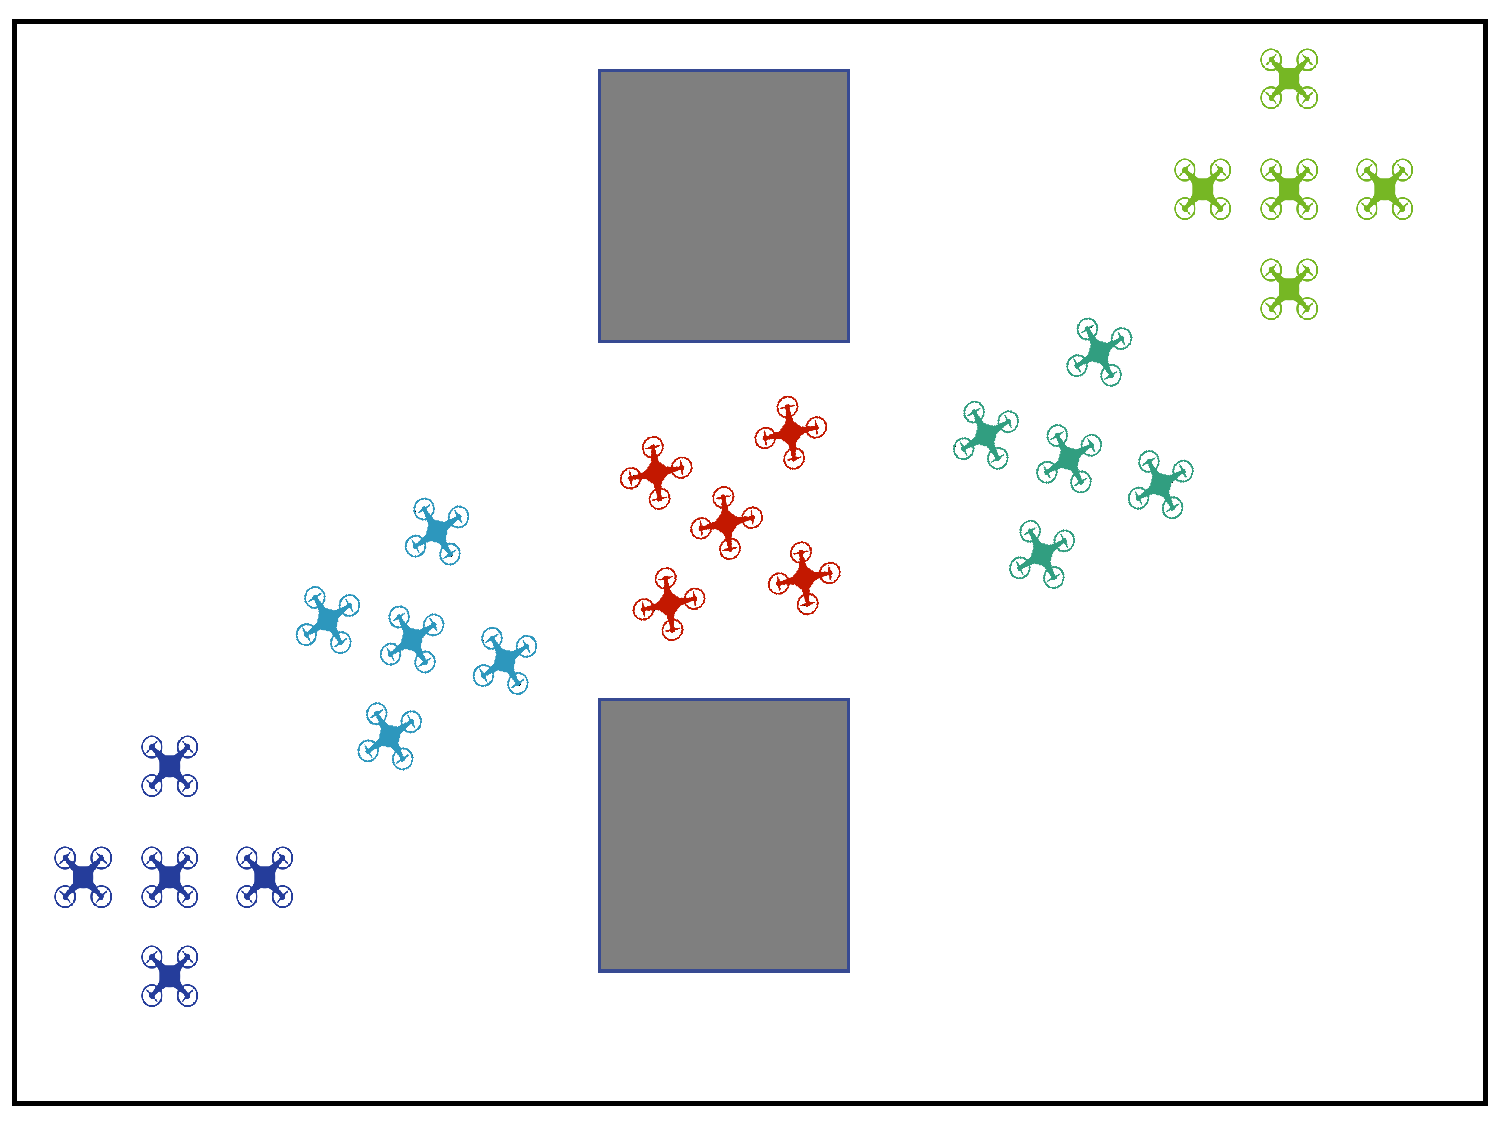
\includegraphics[width=0.45\textwidth]{figures/formation.pdf}
	\caption{Illustration of a (sample) trajectory generated by formally guaranteed feedback controllers for the robot formation control example}
	\label{fig:formation_ex}
\end{figure}

\begin{figure}[t]
	\centering
	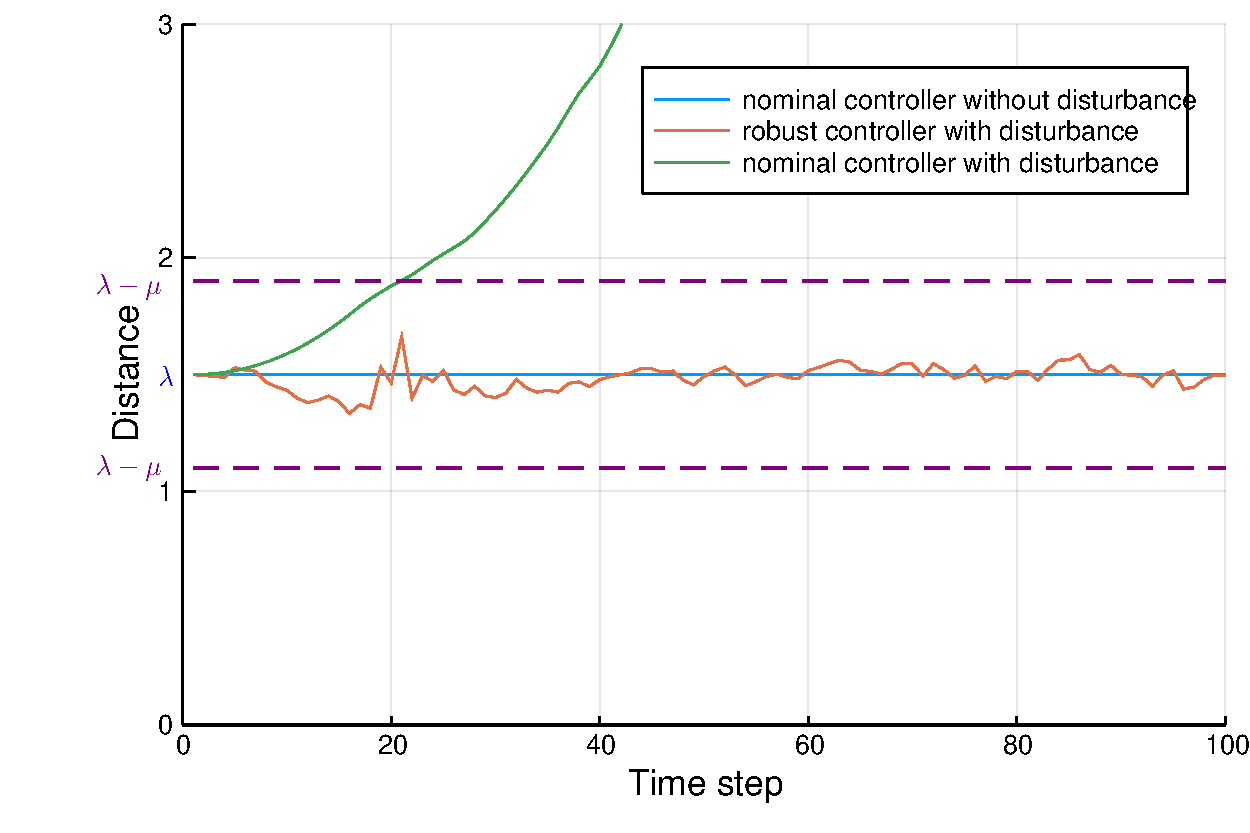
\includegraphics[width=0.45\textwidth]{figures/dist_formation.pdf}
	\caption{Performance of open-loop and feedback controllers in regulating distance between drones for disturbance-free and perturbed situations for the formation control example}
	\label{fig:formation_distance}
\end{figure}
 

%Note that $\delta_{col} > \varepsilon$.
%We use SCOTS in order to synthesize (local) feedback controllers that guarantee reachability, formation control and obstacle/collision avoidance in the presence of bounded disturbance such that $|W|\leq \begin{bmatrix}??&??&??\end{bmatrix}^T$. 
%We consider state and input spaces to be $X=[??:??]^2\times[??,??]$ and
%$U=[??,??]^2$, respectively. Choosing state and input partition sizes $\eta_{X}=[??,??,??]^T$ and
%$\eta_{U}=[??,??]^T$ results in $\hat X$ and $\hat U$ with $??\times ??$ and $??$ points. As we explained in Sec.~\ref{sec:tracking}, we compute the transition system over inter-tube space which has $|\hat P|=??\times ??$ points in this example.%The bound over additive disturbance is set to be $\begin{bmatrix}0.03&0.03&0.03&0\end{bmatrix}^T$. 
%Given the above settings, SCOTS computes abstraction in $??$ minutes for all the drones and synthesizes controllers in about $??$ minutes (in average, abstraction takes $??$ seconds and synthesis takes $??$ seconds). 
%\section{Present Challenges}
%
%\begin{enumerate}
%	\item In some examples, it was necessary to consider a larger control input space for the SCOTS part, than what was used in the ALTRO part.
%	Otherwise, the SCOTS would not be able to track the nominal trajectory within the given precision using any level of discretization. 
%	\item For the ship example, applying the largest disturbance with which SCOTS is able to compute a controller, the trajectory resulted from using the open loop controller does not leave  $\varepsilon-$tube around it; in general magnitude of disturbance for which SCOTS can find a controller is relatively small for most of examples that we have tried.
%\end{enumerate}








